\documentclass{article}

\usepackage[utf8]{inputenc}
\usepackage[T1]{fontenc}
\usepackage{amsmath}
\usepackage{amssymb}
\usepackage{booktabs}
\usepackage{enumitem}
\usepackage{graphicx}
\usepackage{hyperref}
\usepackage{multirow}
\usepackage[verbose=true,letterpaper]{geometry}
\usepackage{times}

\geometry{
  textheight=9in,
  textwidth=5.5in,
  top=1in,
  headheight=12pt,
  headsep=25pt,
  footskip=30pt
}

\setlength{\parindent}{0pt}
\setlength{\parskip}{5.5pt}
\setlist[itemize]{leftmargin=1.5em}
\setlist[enumerate]{leftmargin=1.8em}

\title{AI-DJ: Preference-Based Reinforcement Learning for Automatic DJ Sequencing}

\author{
Neeraja Vasa \\
Hanwen Guo \\
Lilian Pu
}

\begin{document}

\maketitle

\begin{abstract}
Getting a machine to DJ well is not a simple task. Picking the next song requires juggling harmonic compatibility, energy pacing, and transition timing all at once, and hand-written rules for doing this tend to break down across genres and contexts. We present an RL-based AI DJ that learns to sequence tracks using PPO and then attempts to improve that policy with human preference comparisons. The project implements an end-to-end pipeline including a Gymnasium environment over Free Music Archive features, proxy-reward PPO training, pairwise preference collection, Bradley-Terry reward-model training, RLHF fine-tuning, and quantitative evaluation. The final results show that proxy-reward PPO reliably outperforms a random baseline, while RLHF produces mixed outcomes because the learned reward model is limited by a small and noisy preference dataset.
\end{abstract}

\section{Introduction}

DJing is a sequential decision-making task. A good DJ set is not defined only by whether each individual song is good, but by how tracks fit together over time. Tempo changes, energy progression, transition style, repetition, and genre context all affect whether a sequence feels coherent. These criteria are difficult to encode as fixed rules because listener judgments are subjective and depend on the surrounding sequence.

We model this task as simplified DJ sequencing over a track library. At each step, the agent receives a normalized feature vector for the current track and chooses the next track plus a transition type: cut, fade, or beatmatch. The environment is built on Free Music Archive metadata and audio features stored in SQLite. This abstraction does not attempt to synthesize full audio mixes; instead, it focuses on the high-level planning problem of deciding what should come next and how the transition should be treated.

The main challenge is reward design. A purely hand-written reward can encourage useful musical properties such as smooth BPM changes and reasonable energy movement, but it can also overfit to measurable proxies that do not fully capture human taste. To address this, we use a two-stage training pipeline. First, PPO is trained with a proxy reward so that the agent can generate reasonable candidate sequences. Second, human annotators compare generated sequence pairs, and these labels train a reward model that is used for RLHF fine-tuning.

The contribution of this project is an end-to-end prototype for preference-based AI DJ sequencing. The system includes an FMA-backed Gymnasium environment, PPO training, preference-pair generation, a terminal annotation workflow, majority-vote label merging, Bradley-Terry reward-model training, RLHF fine-tuning, and evaluation artifacts. This makes the project a compact but complete testbed for studying how reinforcement learning and human preference feedback can be applied to subjective music sequencing tasks.

\section{Related Work}

Prior work on automatic DJ systems has focused mainly on song mixing and transition generation. MusicMixer uses audio similarity between song sections to suggest and perform seamless mixes for inexperienced users \cite{musicmixer}. Vande Veire and De Bie present a more comprehensive raw-audio DJ system for drum and bass, showing that rule-based and MIR-driven methods can produce full mixes from a local song library \cite{rawaudio}. More recent AI DJ systems combine audience reaction analysis, similarity-based song selection, beatmatching, and equalizer mixing for electronic dance music \cite{aidj}. These systems are closest to the practical goal of our project, but they primarily rely on engineered audio-processing pipelines rather than learning a sequencing policy from preference feedback.

Recent work has also explored playlist sequencing and transition quality beyond traditional recommendation. Liebman et al.\ argue that music preference depends on temporal context, not just isolated song choice, and show that online adaptation to sequential preferences can improve listener experience \cite{rightmusic}. Wang proposes a reinforcement-learning hybrid recommender that models both song preferences and transition preferences \cite{hybridrec}. Tomasi et al.\ develop a simulation-based RL framework for playlist generation, using a modified DQN to optimize user-satisfaction metrics in large action spaces \cite{playlist}. Our work shares this sequential framing, but focuses specifically on DJ-style track selection with explicit transition actions.

Several projects use learning methods directly for DJ automation. Kronvall's DeepFADE system applies hierarchical deep reinforcement learning to music mixing, with separate tiers for song selection, cue-point loading, and transition generation \cite{deepfade}. Its reward functions include beat alignment, volume stability, tonal consonance, and transition timing, but the system suffers from reward hacking and limited policy expressiveness. DJ-AI systems use graph optimization, audio embeddings, and generative models such as MusicGen to arrange playlists and synthesize smoother transitions \cite{djai_sorting,djai_alignment}. Compared with these approaches, our project uses a simpler feature-level environment but directly studies how human preferences can improve the reward signal for sequencing.

Human feedback is especially relevant because musical quality is subjective. Justus applies human-in-the-loop reinforcement learning to music generation, using user feedback as the reward signal for iteratively improving generated compositions \cite{hitl_music}. We apply the same motivation to DJ sequencing rather than composition: instead of asking the agent to create new music, we ask it to choose better sequences of existing tracks. Our contribution is therefore a compact RLHF pipeline for DJ-style sequencing, combining proxy-reward PPO with a Bradley-Terry reward model trained from human pairwise comparisons.

\section{Problem Statement}

A DJ set is a sequence of tracks arranged so that each transition feels natural to listeners. Good sets tend to have smooth tempo changes, coherent energy arcs, and transitions that fit the musical context. Achieving this manually requires experience and intuition that are difficult to encode explicitly. The goal of this work is to automate track sequencing in a way that produces sets a human listener would judge as high quality.

We formalize this as finding an optimal policy $\pi^*$ over a sequence of track selections:
\begin{equation}
    \pi^* = \arg\max_{\pi}\ \mathbb{E}_{\sigma \sim \pi}\left[R(\sigma)\right]
\end{equation}
where $\sigma$ is a full DJ set produced by following policy $\pi$, and $R(\sigma)$ is a measure of overall set quality. The core difficulty is that $R$ is not known in closed form because listener preferences are subjective and context-dependent, so no hand-designed reward function can fully capture what makes a set good. The main technical question is therefore how well a sequencing agent can be trained first with structured proxy rewards and then with a learned reward derived from human judgments.

\section{Method}

The main idea behind our work is simple. People can usually recognize when a DJ set flows well, even if they struggle to explain why. We use this observation to split the problem into two parts. First, we train a policy to generate reasonable track sequences using simple reward signals based on interpretable metrics. Then, we replace or augment those metrics with a reward signal learned directly from human judgments.

\subsection{Environment}

We model track sequencing as a Markov Decision Process using a custom Gymnasium environment. At each step, the agent observes the current track as a normalized feature vector $s_t \in \mathbb{R}^9$ that includes tempo, key, mode, energy, valence, danceability, loudness, chroma mean, and RMS mean. Based on that state, it picks an action $a_t = (\text{track}_{t+1}, \tau_t)$ where $\text{track}_{t+1}$ is the next track chosen from a candidate pool and $\tau_t \in \{\text{cut}, \text{fade}, \text{beatmatch}\}$ determines how the transition is performed. Episodes run for a fixed number of steps over tracks drawn from the Free Music Archive dataset.

\subsection{Stage 1: Proxy Reward Training}

Before collecting human preferences, we need the agent to generate sequences that are worth comparing. To do this, we train a PPO policy using a hand-designed proxy reward based on three basic qualities of a good transition:
\begin{equation}
    r_t = 0.5 \cdot r_{\text{bpm}} + 0.3 \cdot r_{\text{transition}} + 0.2 \cdot r_{\text{energy}} - p_{\text{repeat}}
\end{equation}

The term $r_{\text{bpm}}$ penalizes abrupt tempo jumps between consecutive tracks. The transition reward $r_{\text{transition}}$ captures whether the selected transition type makes sense for the relationship between tracks, for example rewarding beatmatching when BPM differences are small and favoring cuts when energy changes are more dramatic. The energy term encourages sequences that evolve in a musically coherent way rather than moving randomly between intensity levels. We also include a repeat penalty $p_{\text{repeat}}$ to discourage replaying the same track. The policy is a two-layer MLP trained with PPO in Stable Baselines3.

\subsection{Stage 2: Preference Data Collection}

The proxy reward provides a useful starting point, but it misses qualities a human listener cares about. To capture those, we collect pairwise preference labels from human annotators. We generate pairs by rolling out two different policies in the environment. One sequence comes from the trained PPO policy and the other comes from a random policy. This contrast gives annotators a meaningful choice rather than comparing two sequences of similar quality. Any pair containing repeated tracks or very large BPM jumps is filtered out, since those sequences are broken and would only introduce noise to the labels. The A and B sides are randomly assigned to reduce position bias. Annotators choose the sequence with better overall flow, or skip if the choice is genuinely unclear. When multiple annotators label the same pair, we take the majority vote and discard ties.

\subsection{Stage 3: Reward Model Training}

We train a small MLP on winner-loser preference pairs using the Bradley-Terry ranking objective:
\begin{equation}
    \mathcal{L} = -\log \sigma\!\left(R(\sigma_w) - R(\sigma_l)\right)
\end{equation}
Here $\sigma_w$ and $\sigma_l$ are the preferred and rejected sequences, and $R(\cdot)$ is the scalar output of the reward model. Rather than feeding in raw step-by-step features, each sequence is summarized using five aggregate statistics: mean tempo, tempo smoothness, mean energy, energy trend, and beatmatch fraction. This keeps the input small, which matters when the annotation dataset is limited. Training is done with Adam, and we keep the checkpoint with the lowest validation loss.

\subsection{Stage 4: RLHF Fine-Tuning}

Once the reward model is trained, we go back to the Stage 1 PPO checkpoint and continue training against the new signal. In the implementation described in the final analysis, RLHF uses a terminal reward from the learned preference model; the broader design also supports mixing that learned reward with the original proxy reward to keep the policy grounded in transition-level structure. The goal is to optimize long-run sequence quality as judged by human preferences without discarding the local musical constraints that made the proxy-trained policy workable in the first place.

\section{Experimental Design}

We study automatic DJ sequencing as a sequential decision-making problem. Given the current track, an agent chooses the next track and a transition type. The environment is built from Free Music Archive data stored in `fma\_db/data/fma.db`, with track-level features such as tempo, key, energy, valence, danceability, loudness, chroma, and RMS.

The project tests three hypotheses:
\begin{itemize}
\item H1: PPO trained on the proxy reward in `DJEnv` will outperform a random policy.
\item H2: Larger PPO runs will improve policy quality, although the learned policy may still trail a greedy heuristic baseline.
\item H3: RLHF fine-tuning with a learned reward model can improve a proxy-trained PPO checkpoint, but only if the reward model generalizes well.
\end{itemize}

The proxy reward used for PPO is
\[
0.5 \cdot \text{bpm\_smoothness} + 0.3 \cdot \text{transition\_reward} + 0.2 \cdot \text{energy\_flow} - \text{repeat\_penalty}.
\]
This reward encourages smooth tempo changes, context-appropriate transitions, coherent energy flow, and avoidance of repeated tracks. For RLHF, the proxy reward is replaced by or paired with a terminal reward from the learned preference model depending on the experiment configuration.

The main experiments use a 500-track subset, 12-step episodes, and a human-preference dataset built from 50 generated sequence pairs. Three annotators labeled these pairs; after majority voting, 43 usable preference examples remained, 7 ties were dropped, and pairwise agreement was 0.5982.

We ran three experiments:
\begin{enumerate}
\item PPO vs.\ random: test whether PPO beats the random baseline and shows an upward learning curve.
\item PPO scaling and heuristic comparison: compare saved PPO runs at increasing timestep budgets and measure the gap to the heuristic baseline.
\item RLHF fine-tuning: start from a PPO checkpoint, train a reward model on merged preference labels, then fine-tune PPO with terminal reward from that model.
\end{enumerate}

The evaluation criteria are straightforward. For H1, PPO must exceed the random baseline and show upward reward trends. For H2, larger PPO runs should improve reward and ideally narrow the gap to the heuristic policy. For H3, RLHF should improve the starting PPO checkpoint on proxy reward, learned reward, or direct human preference; the saved repository mainly supports the first two.

\section{Results and Discussion}

\subsection{Core Results}

\begin{table}[t]
\centering
\caption{Preference-data and reward-model summary.}
\begin{tabular}{ll}
\toprule
Result & Value \\
\midrule
Preference pairs generated & 50 \\
Usable merged preference pairs & 43 \\
Pairwise annotator agreement & 0.5982 \\
Reward-model best validation epoch & 1 \\
Reward-model best validation loss & 0.7070 \\
\bottomrule
\end{tabular}
\end{table}

\begin{table}[t]
\centering
\caption{Main PPO and RLHF evaluation runs.}
\small
\begin{tabular}{llllll}
\toprule
Run & Timesteps & Random & Heuristic & Score & Improvement \\
\midrule
`ppo\_smoke` & 2,048 & 8.1183 & n/a & 8.4567 & +0.3384 vs random \\
`ppo\_20260406\_220618` & 16,384 & 8.4582 & n/a & 9.3478 & +0.8896 vs random \\
`ppo\_20260410\_002422` & 65,536 & 7.8289 & 11.2695 & 10.2409 & +2.4120 vs random \\
`ppo\_20260413\_004855` & 65,536 & 7.4781 & 11.3320 & 8.0709 & +0.5928 vs random \\
`rlhf\_20260413\_000436` & 32,768 & start 9.9051 & n/a & 9.1785 & -0.7266 vs start \\
`rlhf\_20260413\_005446` & 32,768 & start 8.1051 & n/a & 8.2579 & +0.1528 vs start \\
\bottomrule
\end{tabular}
\end{table}

% \subsection{Figures}

% \begin{figure}[t]
% \centering
% 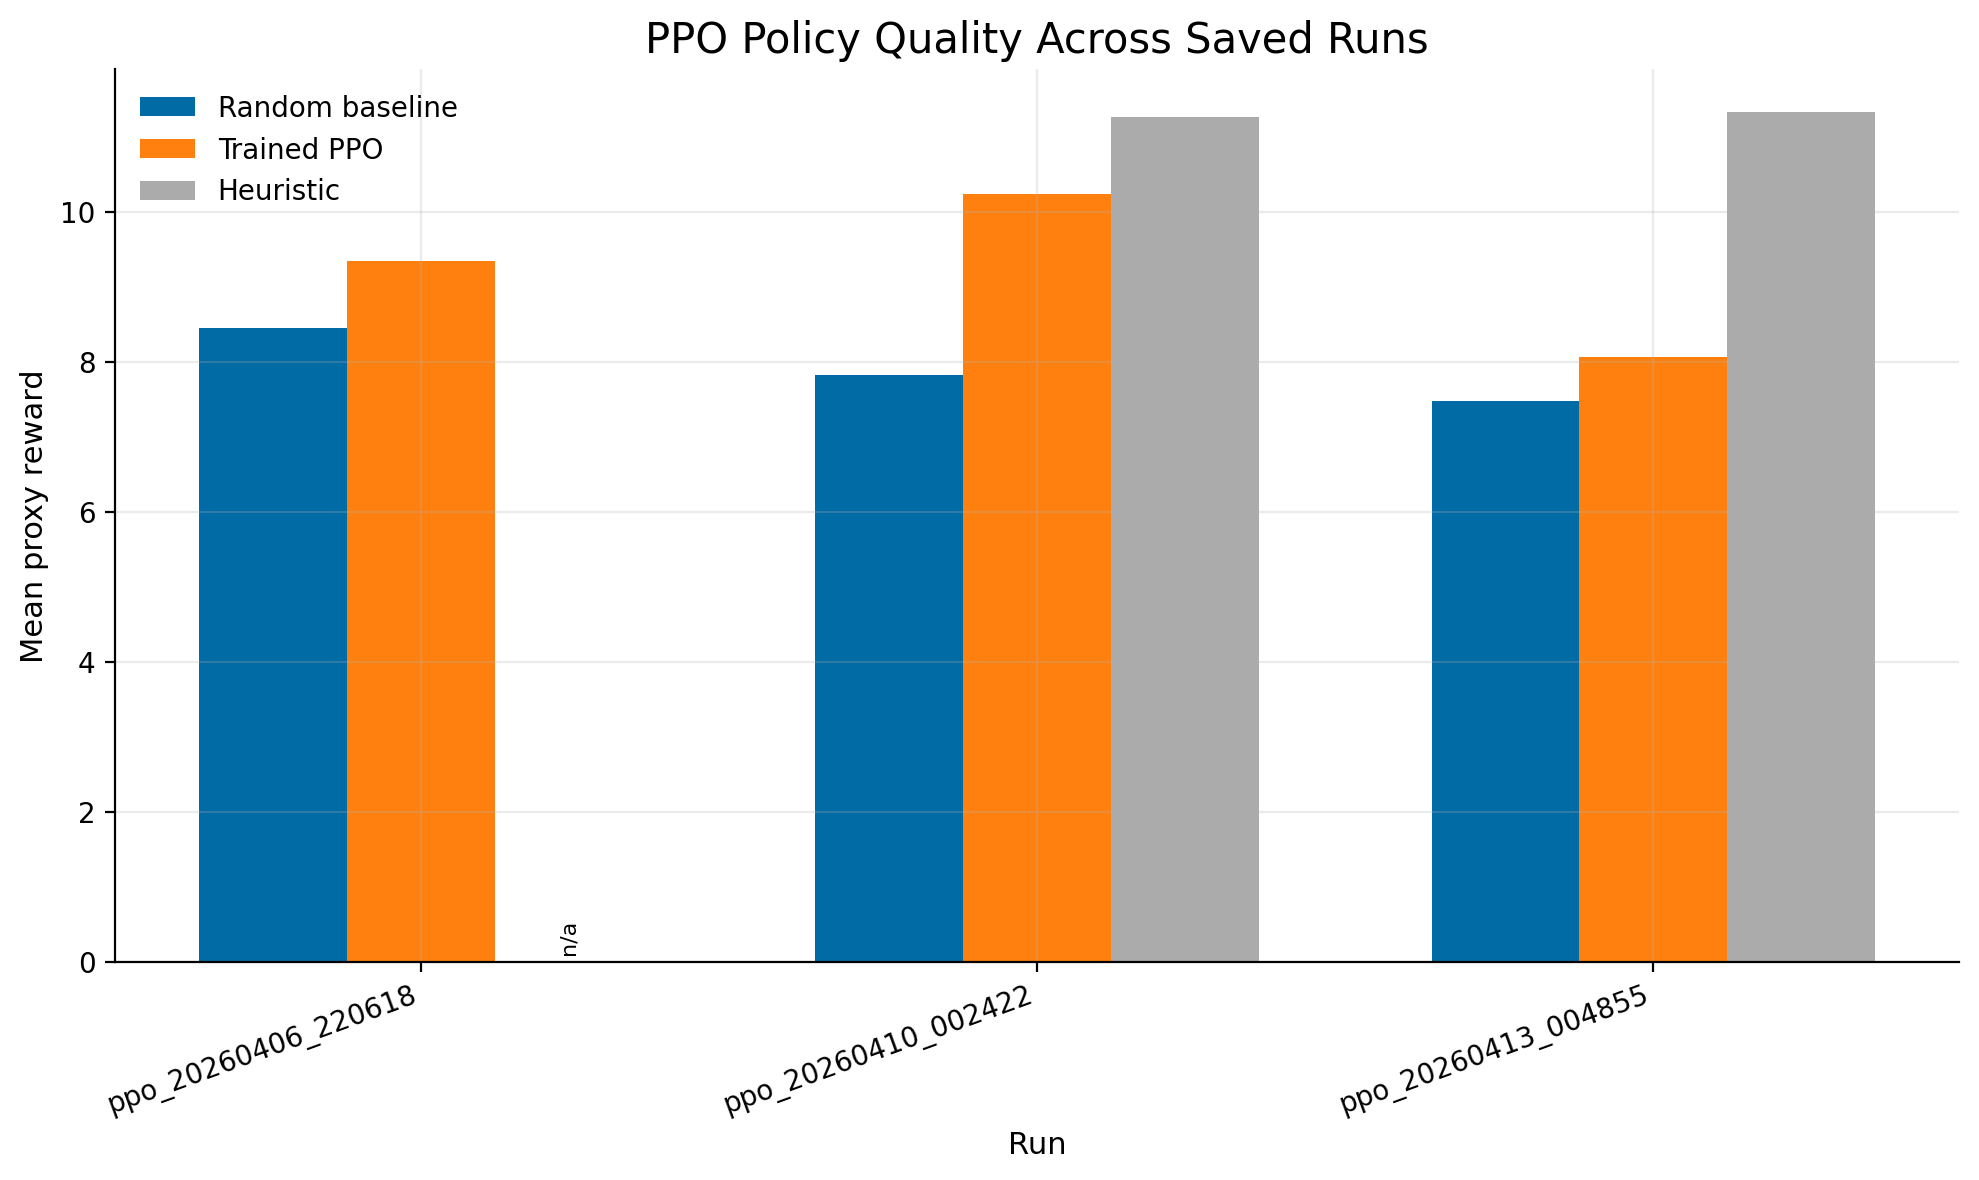
\includegraphics[width=\linewidth]{../graphs/ppo_run_comparison.png}
% \caption{Comparison of saved PPO runs against the random and heuristic baselines.}
% \label{fig:ppo-comparison}
% \end{figure}

% \begin{figure}[t]
% \centering
% 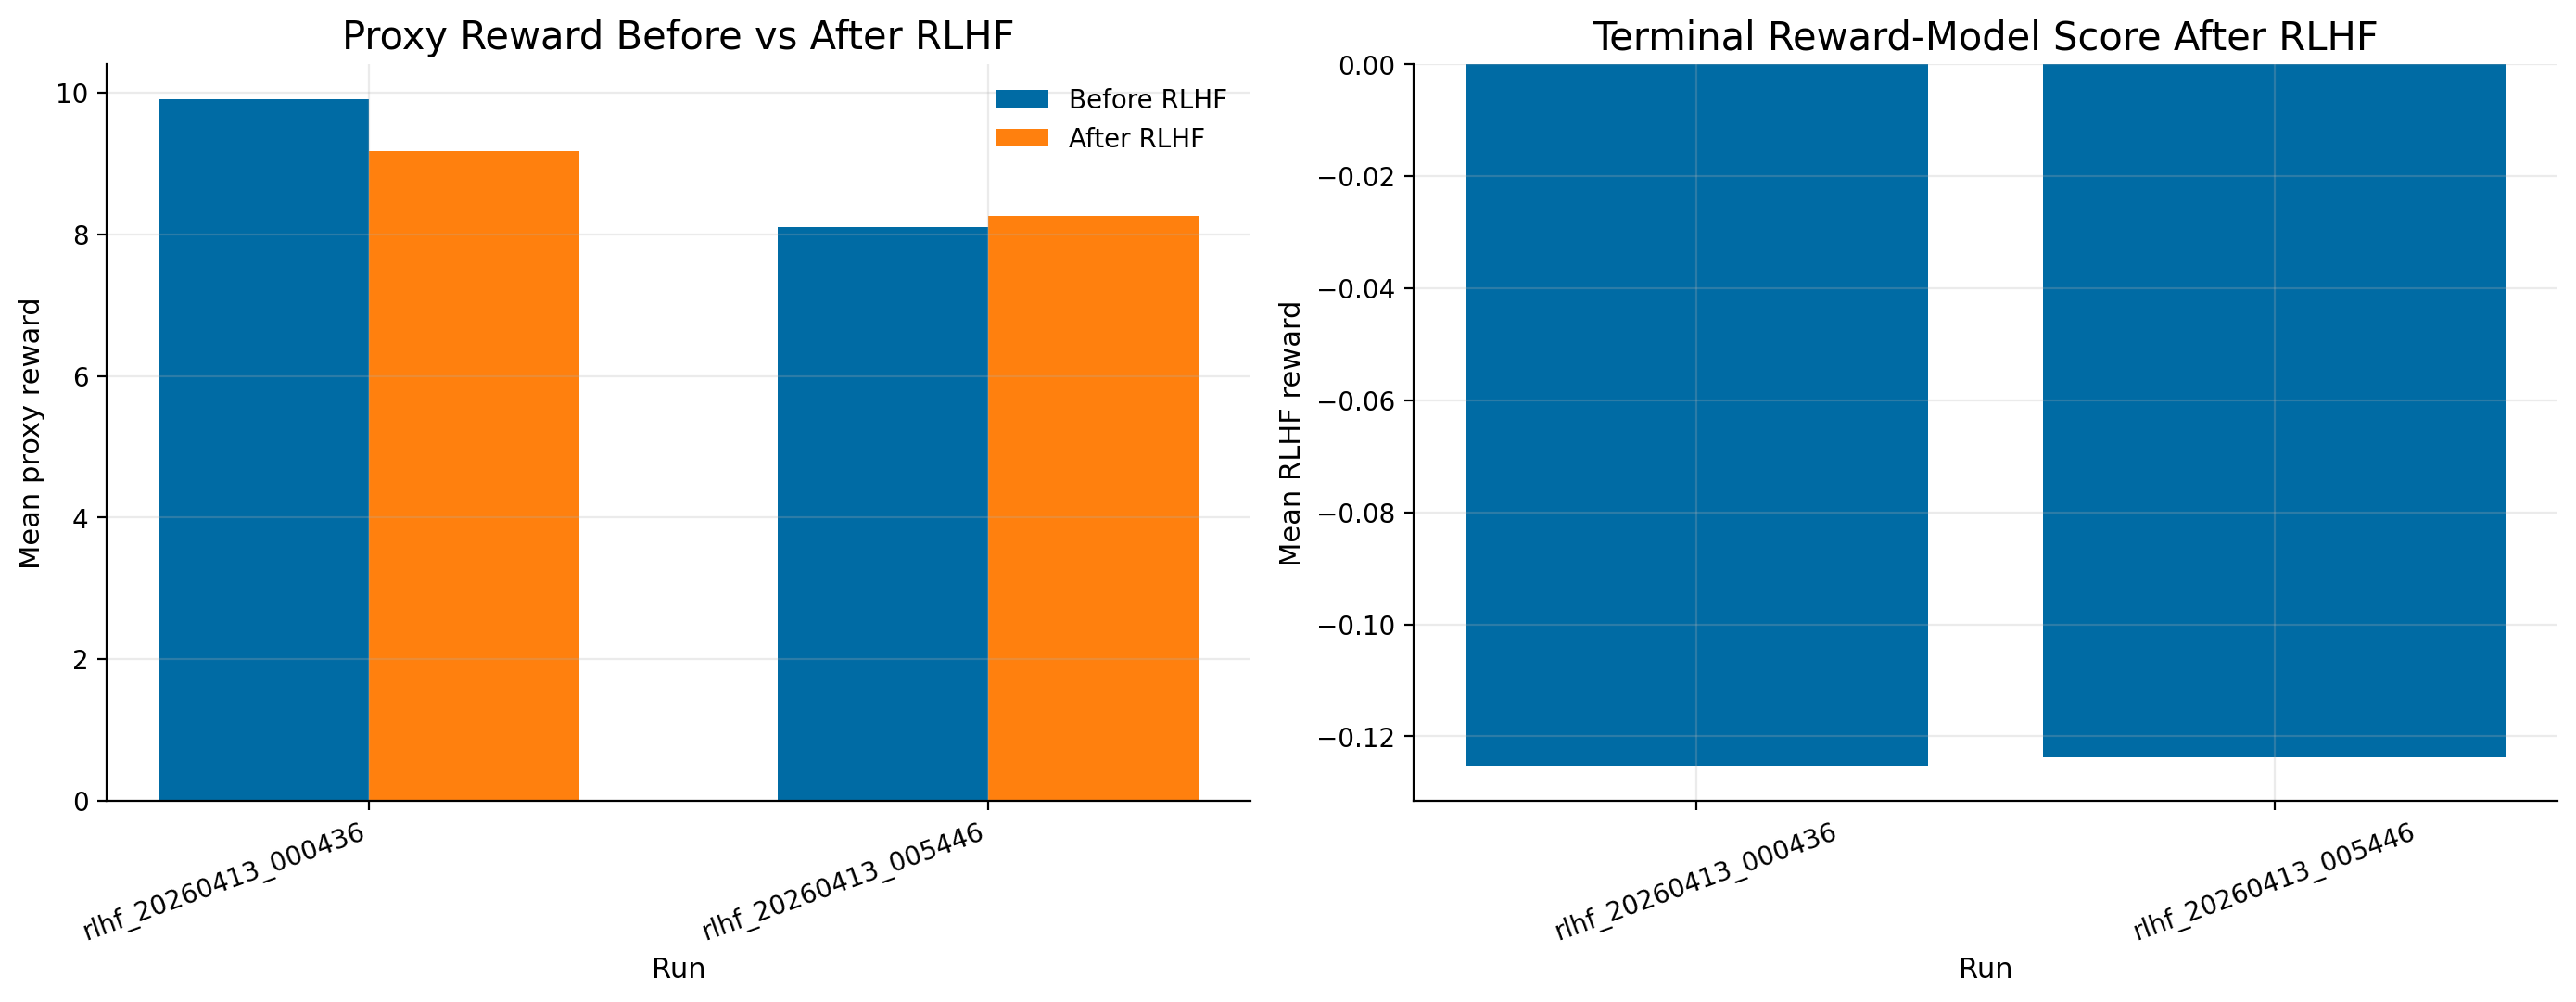
\includegraphics[width=\linewidth]{../graphs/rlhf_run_comparison.png}
% \caption{Comparison of RLHF fine-tuning runs relative to their starting PPO checkpoints.}
% \label{fig:rlhf-comparison}
% \end{figure}

% \begin{figure}[t]
% \centering
% 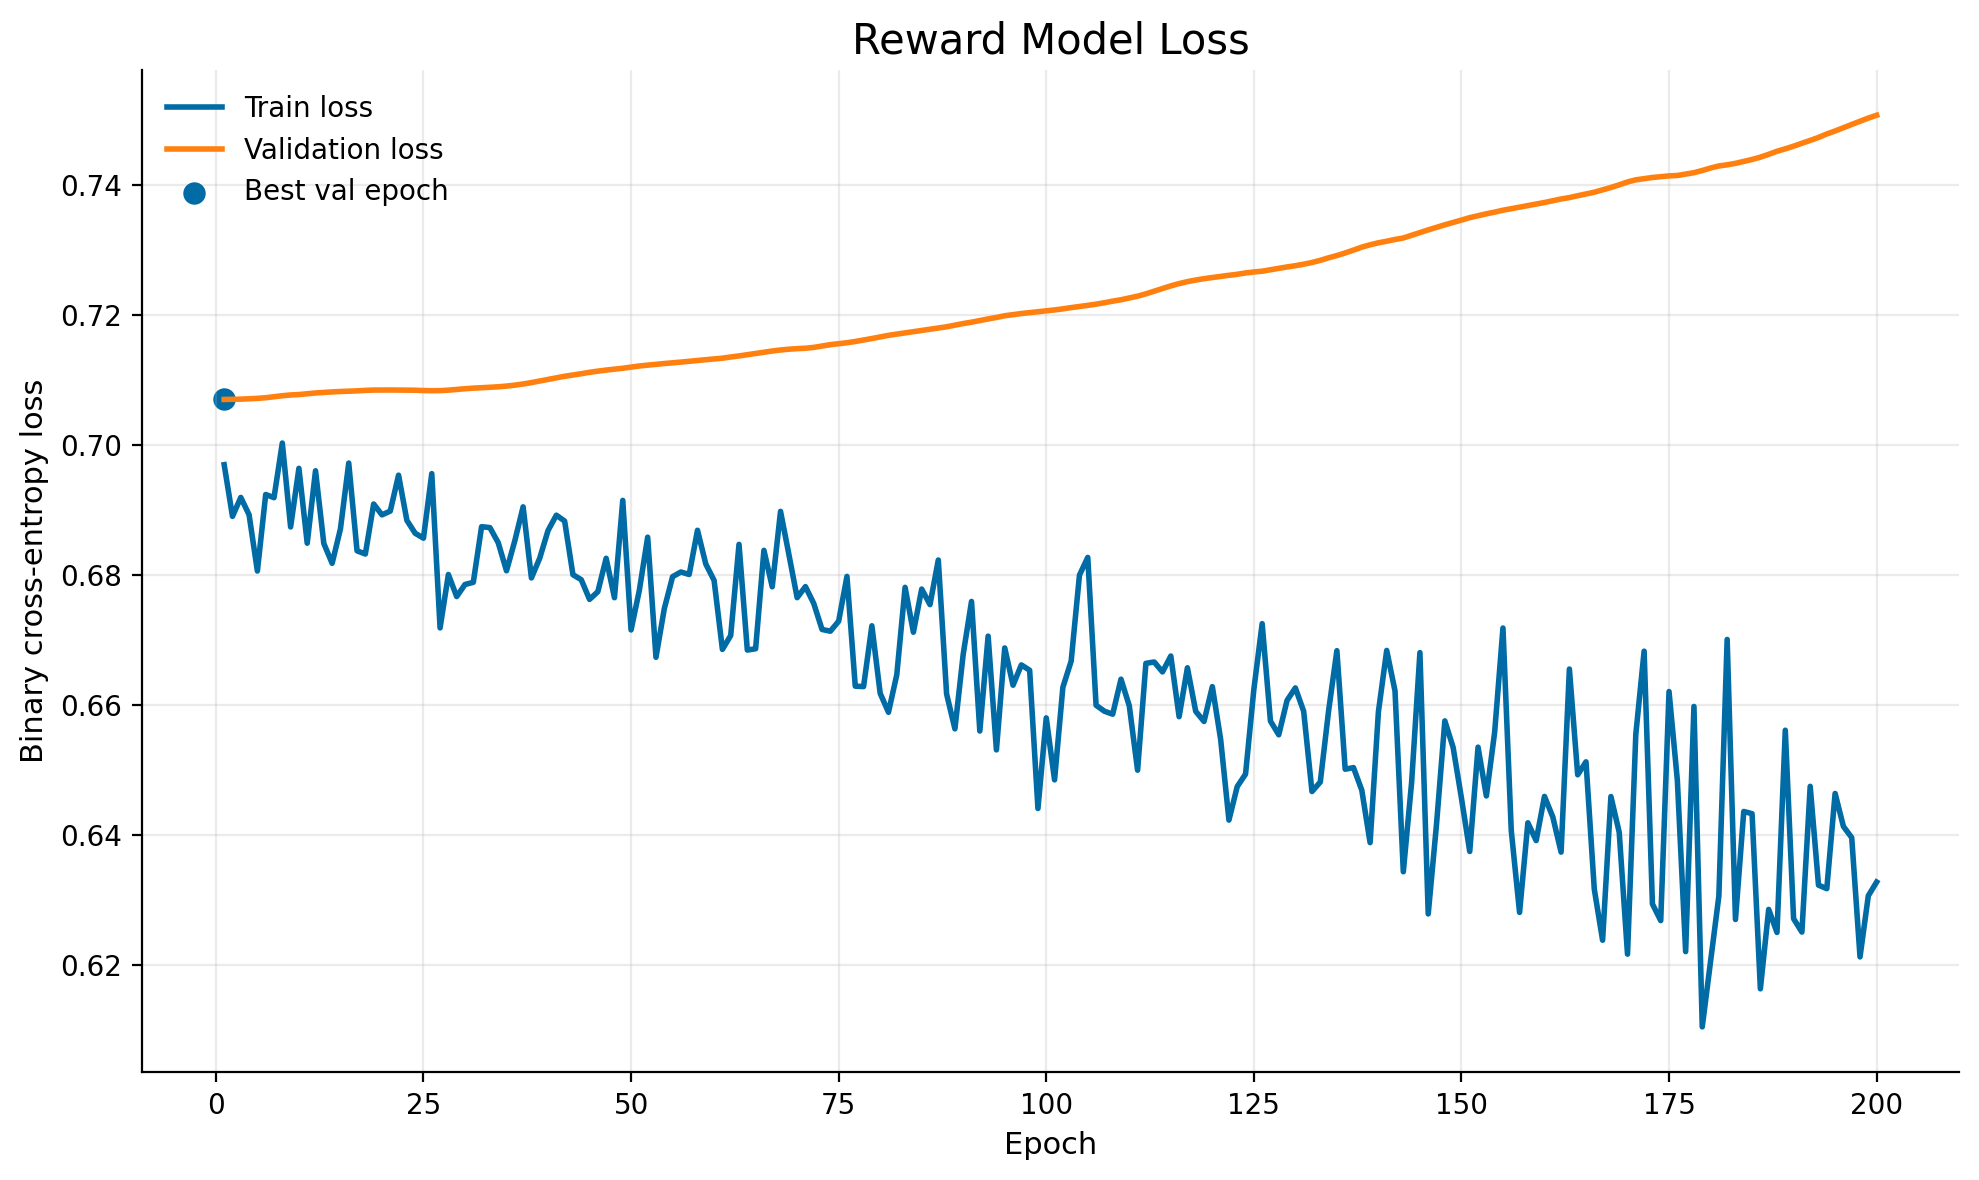
\includegraphics[width=\linewidth]{../graphs/reward_model_loss.png}
% \caption{Reward-model training and validation loss, showing the best validation performance at epoch 1.}
% \label{fig:reward-model-loss}
% \end{figure}


\subsection{Analysis}

The strongest result is that PPO consistently beats random, which supports H1. All saved PPO runs improve on the random baseline and show upward learning curves. The best PPO checkpoint, `ppo\_20260410\_002422`, reaches 10.2409, a gain of 2.4120 over random. This shows that the proxy-reward environment is learnable and that the PPO pipeline works end to end.

H2 is partially supported. Increasing training scale improves the best observed PPO result, but performance is not stable across runs. Two runs with the same 65,536 timestep budget differ sharply: one reaches 10.2409, while the later run reaches only 8.0709. This suggests sensitivity to seed, initialization, or training variance. In addition, PPO still trails the heuristic baseline, which stays near 11.3. The learned policy is useful, but it has not surpassed the strongest hand-designed strategy under the same proxy objective.

H3 is also only partially supported. One RLHF run improves its starting PPO checkpoint slightly, from 8.1051 to 8.2579, but another degrades substantially, from 9.9051 to 9.1785. The RLHF effect is therefore not robust. The most likely reason is the reward model: its best validation loss occurs at epoch 1, and validation loss worsens afterward despite lower training loss. That pattern indicates overfitting or weak supervision.

The reward-model bottleneck is consistent with the dataset size. The reward model was trained from only 43 usable preference pairs, and human agreement was moderate rather than high. That is enough to prove the pipeline works, but not enough to provide a strong, stable learning signal for RLHF. The current results therefore suggest that proxy-reward PPO is the strongest component of the system, while RLHF is limited primarily by reward-model quality.

\subsection{Follow-On Experiments}

Three follow-on experiments deepen this interpretation:
\begin{enumerate}
\item PPO scaling: comparing 2,048, 16,384, and 65,536 timesteps shows that more training can help substantially, but also exposes variance across large runs.
\item Different RLHF starting checkpoints: the two RLHF runs suggest that a weak reward model can either slightly help or actively hurt an existing PPO policy depending on the starting point.
\item Reward-model diagnostics: the validation-loss curve itself is a critical follow-on experiment because it localizes the main problem to preference modeling rather than PPO implementation.
\end{enumerate}

Overall, the results confirm that the system works technically, but they do not yet show that RLHF reliably outperforms the best PPO-only policy.

\section{Conclusion and Future Work}

This project explored AI DJ sequencing with PPO and RLHF. The main problem is interesting because good DJ behavior depends on both objective transition quality and subjective human judgments of flow. That makes it a natural domain for combining reinforcement learning with preference learning.

The main finding is that PPO successfully learns meaningful sequencing behavior from a structured proxy reward, consistently outperforming a random baseline. A second important finding is that RLHF is not yet reliable in the current system. It can produce small gains, but it can also degrade a strong starting checkpoint. The clearest explanation is that the reward model was trained on too little and too noisy preference data.

We learned three main lessons:
\begin{itemize}
\item Proxy rewards are strong enough to make the task learnable.
\item RLHF quality depends more on reward-model supervision than on PPO itself.
\item Small preference datasets are not enough to consistently beat the best proxy-trained policy.
\end{itemize}

With another month or two, the most important next steps would be:
\begin{enumerate}
\item Collect several hundred preference pairs instead of a few dozen.
\item Improve annotation consistency with better instructions and calibration.
\item Train a stronger reward model, ideally one that models sequence structure more explicitly.
\item Run larger held-out human evaluations comparing PPO directly to RLHF.
\item Stabilize PPO with repeated seeds and more systematic checkpoint selection.
\item Explore hybrid training that mixes proxy reward and learned reward instead of replacing the proxy reward entirely.
\end{enumerate}

In short, the project already demonstrates a complete AI DJ pipeline, but its most important scientific result is that the hard part is not getting PPO to learn. The hard part is learning a reward model from human preferences that is strong enough to guide further improvement.

\begin{thebibliography}{9}

\bibitem{musicmixer}
Tatsunori Hirai, Hironori Doi, and Shigeo Morishima.
\newblock MusicMixer: Computer-aided DJ system based on an automatic song mixing.
\newblock In \emph{Proceedings of the 12th International Conference on Advances in Computer Entertainment Technology}, 2015.

\bibitem{aidj}
Hao-Wei Huang, Muhammad Fadli, Achmad Kripton Nugraha, Chih-Wei Lin, and Ray-Guang Cheng.
\newblock AI DJ System for Electronic Dance Music.
\newblock In \emph{International Symposium on Electronics and Smart Devices}, 2022.

\bibitem{hitl_music}
Aju Ani Justus.
\newblock Music Generation Using Human-In-The-Loop Reinforcement Learning.
\newblock In \emph{IEEE International Conference on Big Data}, 2023.

\bibitem{deepfade}
Viktor Kronvall.
\newblock \emph{Mixing Music Using Deep Reinforcement Learning}.
\newblock Master's thesis, 2019.

\bibitem{djai_alignment}
Orkun Kinay, Baris Tekdemir, Goktug Gokyilmaz, Ekmel Yavuz, Berk Ay, and Selim Balcisoy.
\newblock DJ AI: Optimizing playlist alignment and generating transitions with generative and embedding models.
\newblock In \emph{International Audio Mostly Conference}, 2025.

\bibitem{djai_sorting}
Orkun Kinay, Baris Tekdemir, Goktug Gokyilmaz, Ekmel Yavuz, Berk Ay, and Selim Balcisoy.
\newblock DJ-AI: Intelligent playlist sorting and seamless generative transitions.
\newblock In \emph{Signal Processing and Communications Applications Conference}, 2025.

\bibitem{rightmusic}
Elad Liebman, Maytal Saar-Tsechansky, and Peter Stone.
\newblock The right music at the right time: Adaptive personalized playlists based on sequence modeling.
\newblock \emph{MIS Quarterly}, 43(3), 2019.

\bibitem{playlist}
Federico Tomasi, Joseph Cauteruccio, Surya Kanoria, Kamil Ciosek, Matteo Rinaldi, and Zhenwen Dai.
\newblock Automatic music playlist generation via simulation-based reinforcement learning.
\newblock In \emph{Proceedings of the 29th ACM SIGKDD Conference on Knowledge Discovery and Data Mining}, 2023.

\bibitem{rawaudio}
Len Vande Veire and Tijl De Bie.
\newblock From raw audio to a seamless mix: Creating an automated DJ system for drum and bass.
\newblock \emph{EURASIP Journal on Audio, Speech, and Music Processing}, 2018.

\bibitem{hybridrec}
Yu Wang.
\newblock A hybrid recommendation for music based on reinforcement learning.
\newblock In \emph{Advances in Knowledge Discovery and Data Mining}, 2020.

\end{thebibliography}

\newpage

\subsection{Figures}

\begin{figure}[t]
\centering
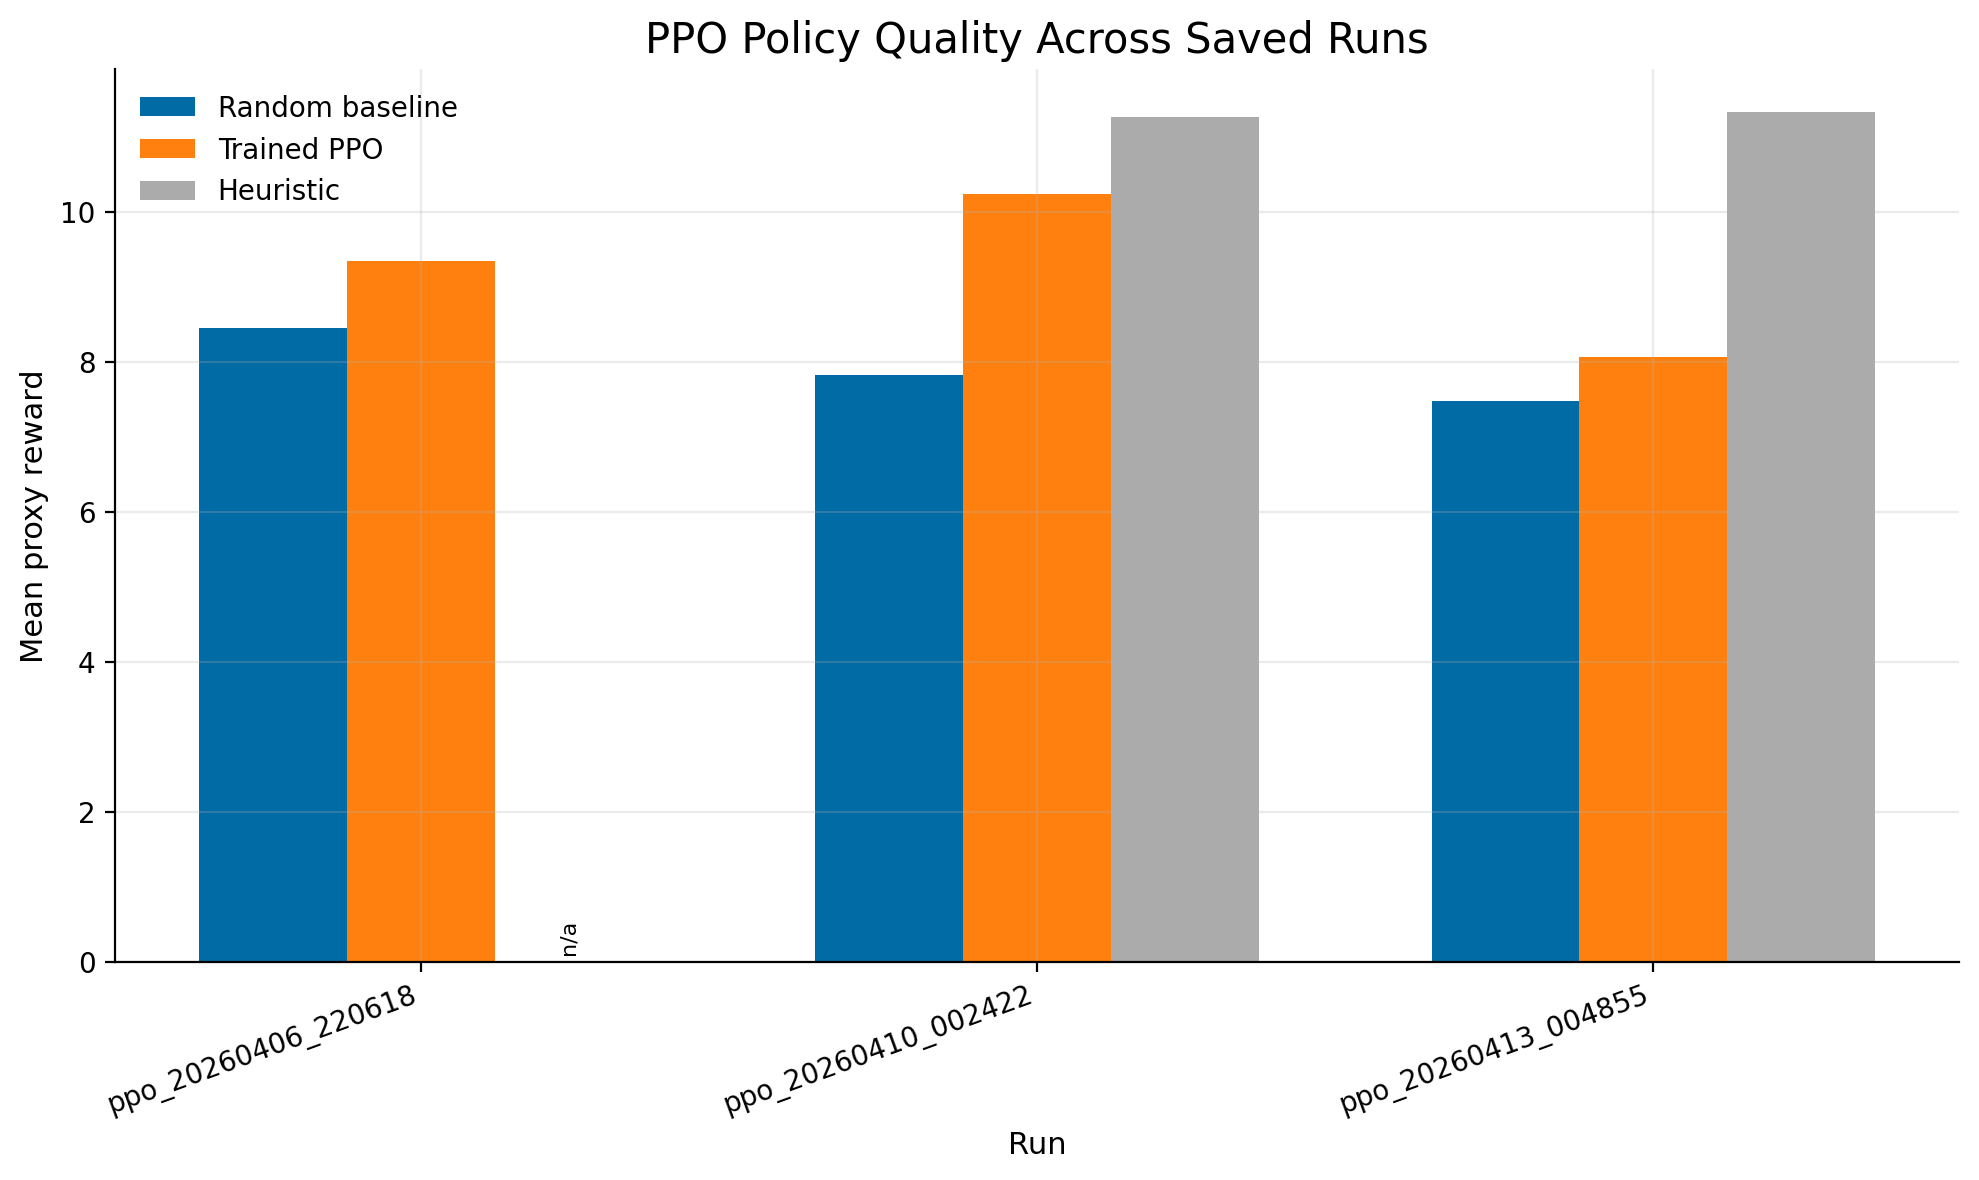
\includegraphics[width=\linewidth]{../graphs/ppo_run_comparison.png}
\caption{Comparison of saved PPO runs against the random and heuristic baselines.}
\label{fig:ppo-comparison}
\end{figure}

\begin{figure}[t]
\centering
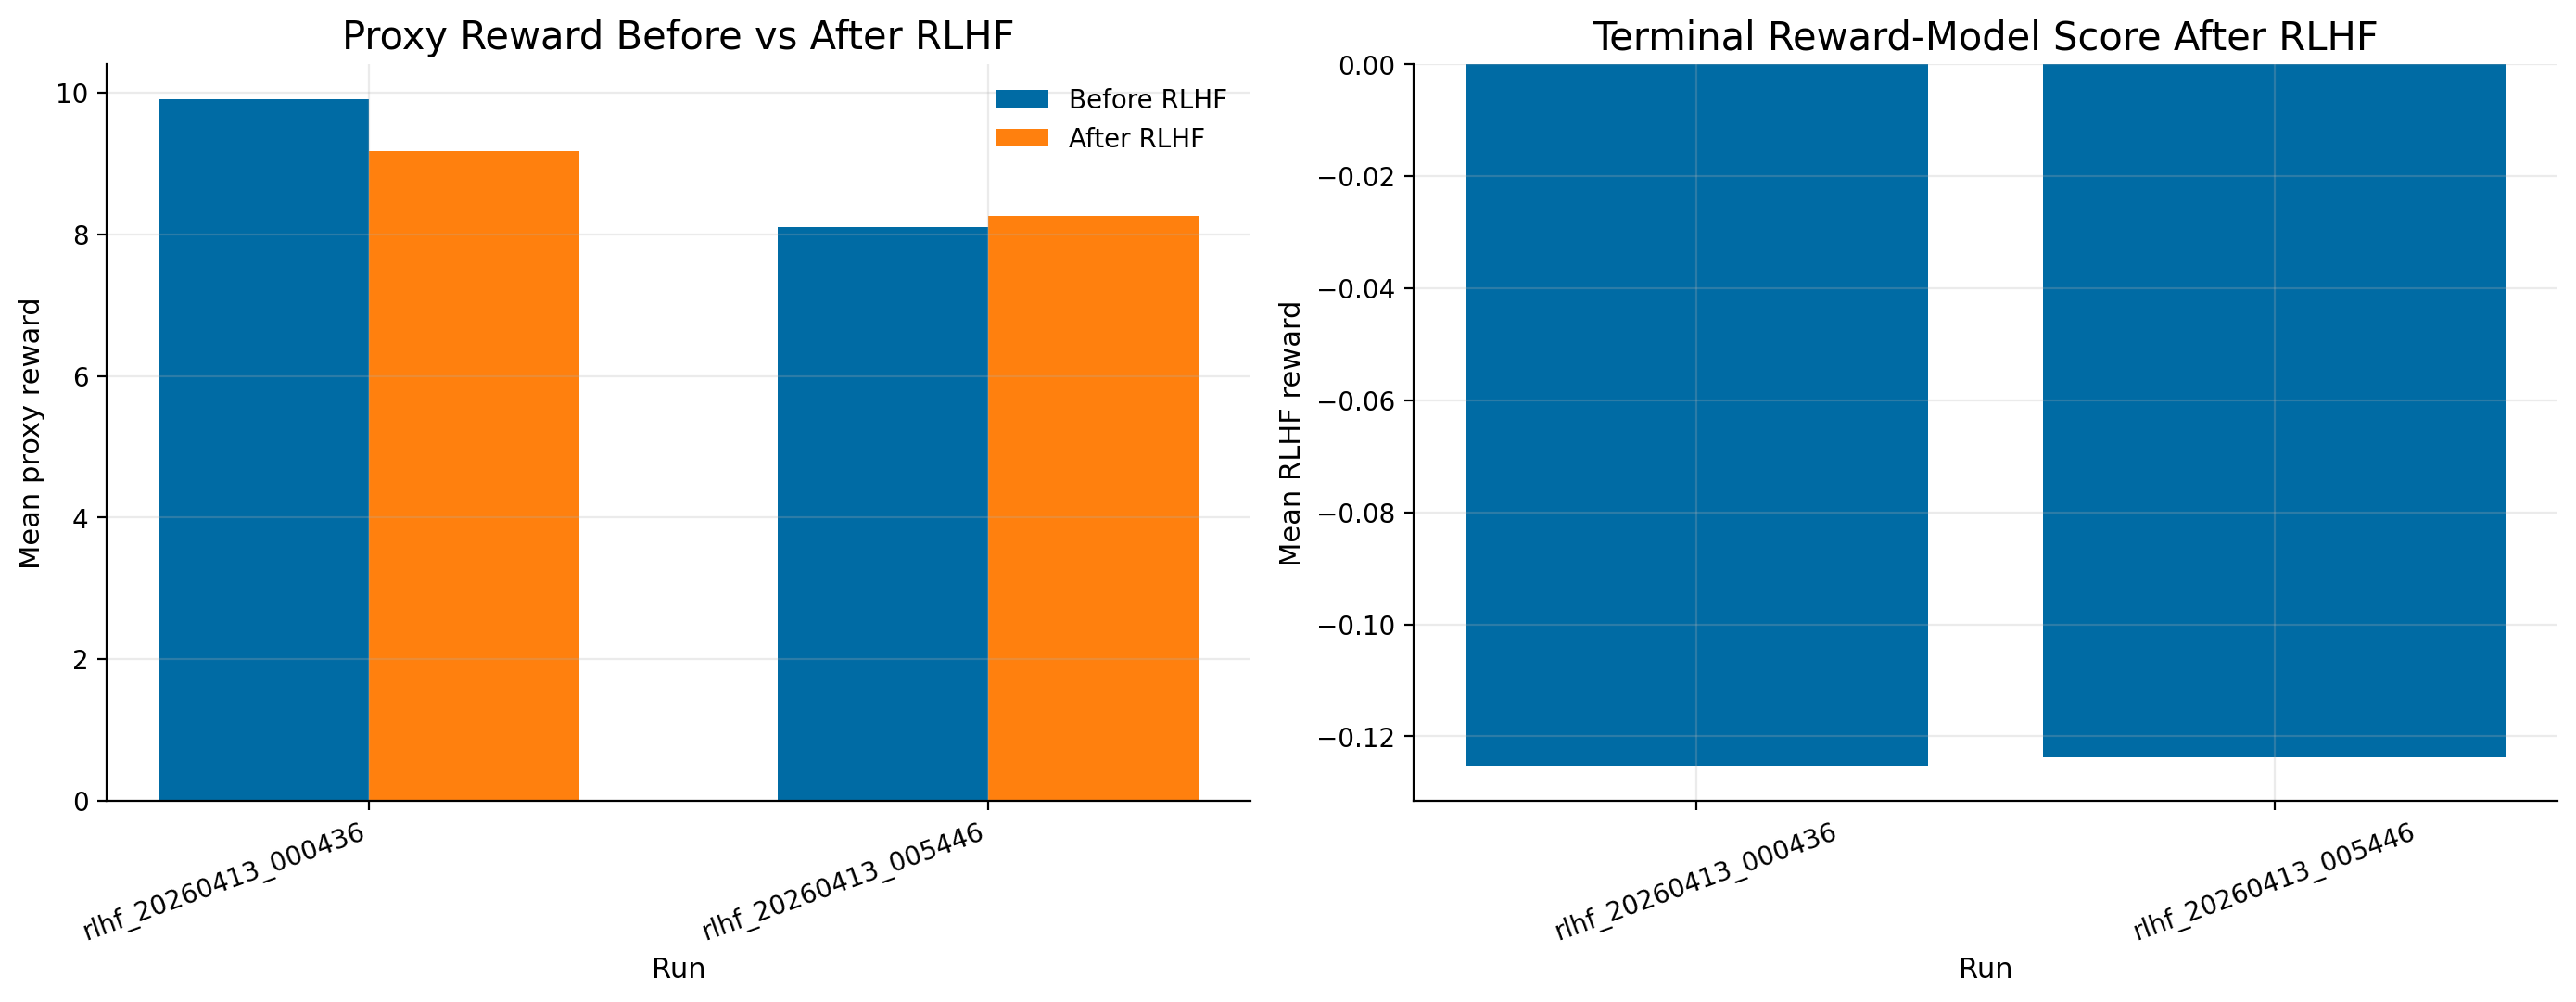
\includegraphics[width=\linewidth]{../graphs/rlhf_run_comparison.png}
\caption{Comparison of RLHF fine-tuning runs relative to their starting PPO checkpoints.}
\label{fig:rlhf-comparison}
\end{figure}

\begin{figure}[t]
\centering
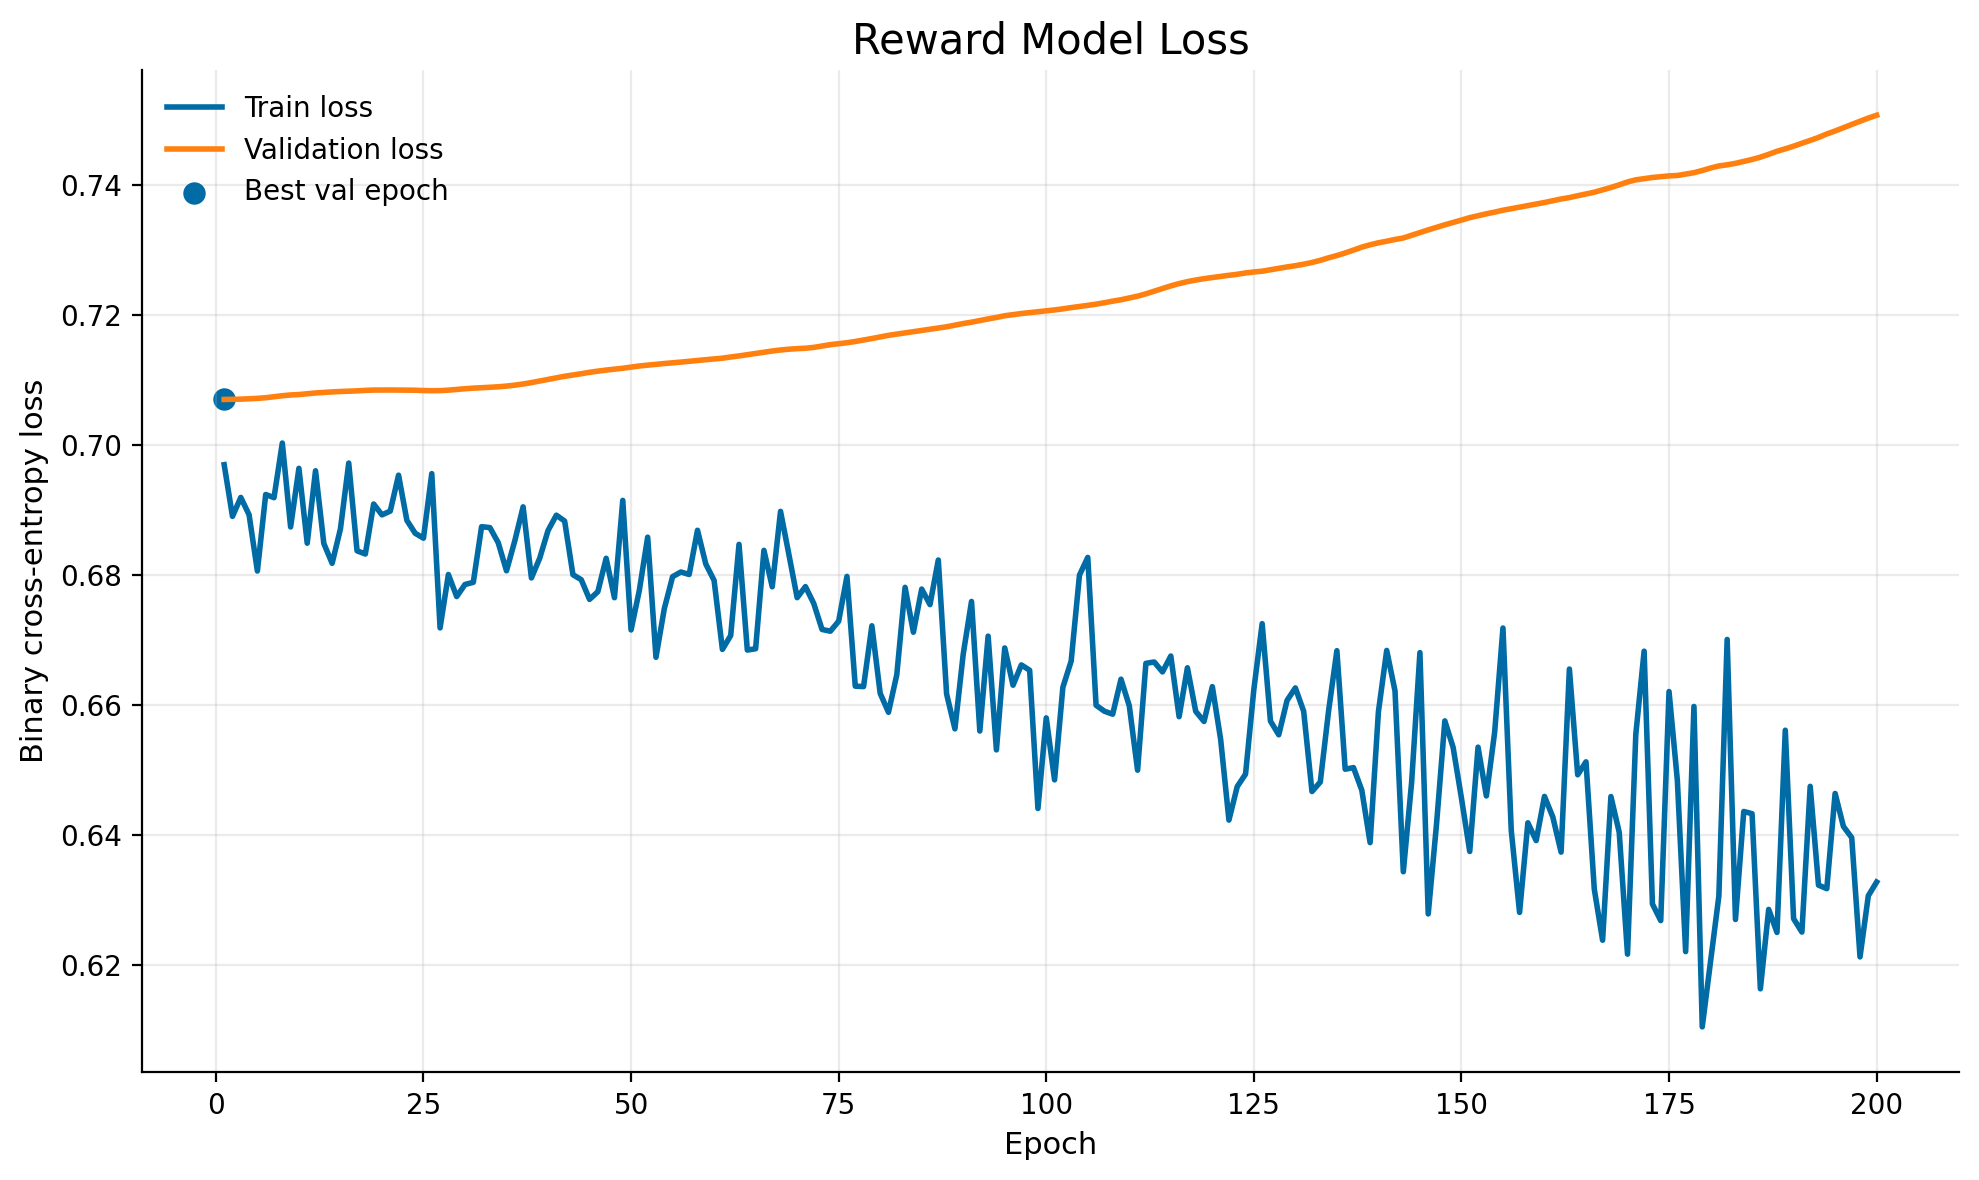
\includegraphics[width=\linewidth]{../graphs/reward_model_loss.png}
\caption{Reward-model training and validation loss, showing the best validation performance at epoch 1.}
\label{fig:reward-model-loss}
\end{figure}


\end{document}
